\documentclass[dvipdfmx]{jarticle}
\pagestyle{empty}
\usepackage{tikz}
\usepackage[utf8]{inputenc}
\usetikzlibrary{shapes,calc}
\newcommand{\lparen}{`\texttt{(}'}
\newcommand{\rparen}{`\texttt{)}'}
\newcommand{\tcomma}{`\texttt{,}'}
\begin{document}
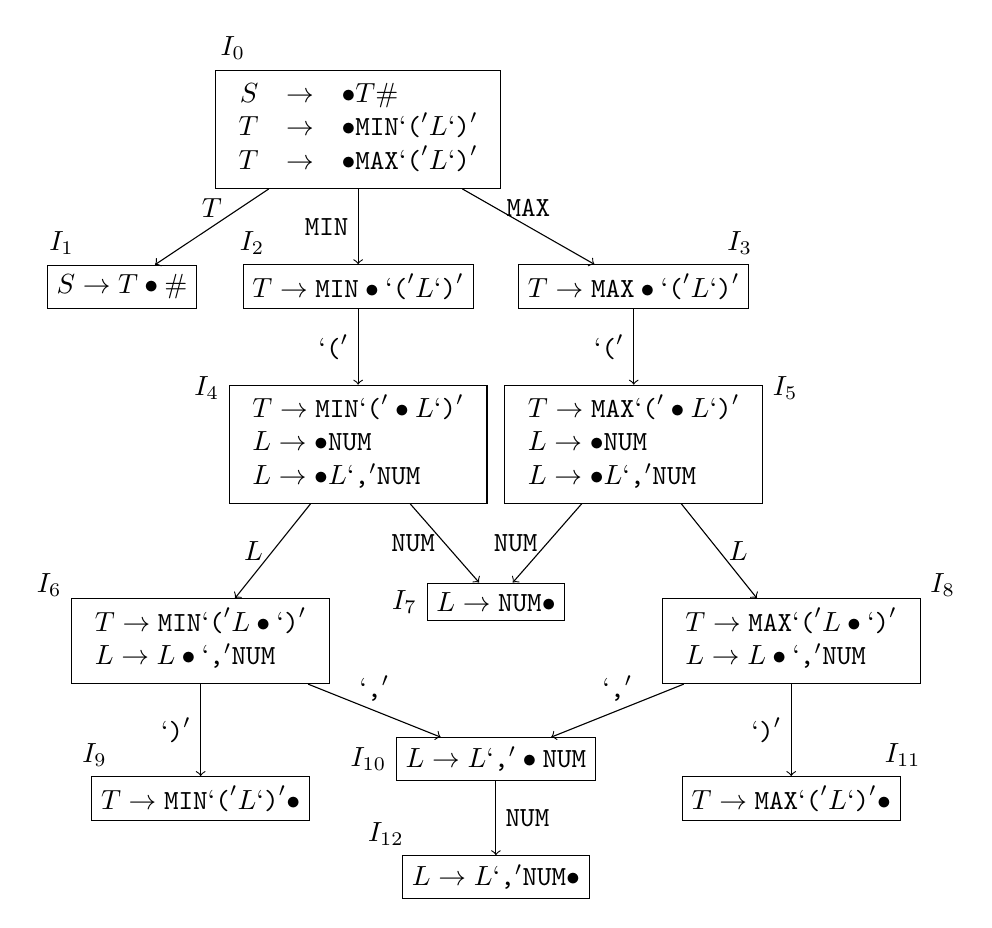
\begin{tikzpicture}
  \node[draw,rectangle,label=150:{$I_0$}] (I0) at (0,0) {$\begin{array}{rcl}
    S & \rightarrow & \bullet T\#\\
    T & \rightarrow & \bullet\texttt{MIN} \lparen L \rparen\\
    T & \rightarrow & \bullet\texttt{MAX} \lparen L \rparen 
  \end{array}$};
  \node[draw,rectangle,label=150:{$I_1$}] (I1) at ($(I0)+(-3,-2)$)
  {$S\rightarrow T\bullet\#$};
  \node[draw,rectangle,label=165:{$I_2$}] (I2) at ($(I0)+(0,-2)$)
  {$T\rightarrow\texttt{MIN}\bullet\lparen L\rparen$};
  \node[draw,rectangle,label=15:{$I_3$}] (I3) at ($(I0)+(3.5,-2)$)
  {$T\rightarrow\texttt{MAX}\bullet\lparen L\rparen$};
  \node[draw,rectangle,label=165:{$I_4$}] (I4) at ($(I2)+(0,-2)$)
  {$\begin{array}{l}T\rightarrow\texttt{MIN}\lparen\bullet L\rparen\\
    L\rightarrow\bullet\texttt{NUM}\\
    L\rightarrow\bullet L\tcomma\texttt{NUM}\end{array}$};
  \node[draw,rectangle,label=15:{$I_5$}] (I5) at ($(I3)+(0,-2)$)
  {$\begin{array}{l}T\rightarrow\texttt{MAX}\lparen\bullet L\rparen\\
    L\rightarrow\bullet\texttt{NUM}\\
    L\rightarrow\bullet L\tcomma\texttt{NUM}\end{array}$};
  \node[draw,rectangle,label=165:{$I_6$}] (I6) at ($(I4)+(-2,-2.5)$)
  {$\begin{array}{l}T\rightarrow\texttt{MIN}\lparen L\bullet\rparen\\
    L\rightarrow L\bullet\tcomma\texttt{NUM}\end{array}$};
  \node[draw,rectangle,label=180:{$I_7$}] (I7) at ($(I4)+(1.75,-2)$)
  {$L\rightarrow\texttt{NUM}\bullet$};
  \node[draw,rectangle,label=15:{$I_8$}] (I8) at ($(I5)+(2,-2.5)$)
  {$\begin{array}{l}T\rightarrow\texttt{MAX}\lparen L\bullet\rparen\\
    L\rightarrow L\bullet\tcomma\texttt{NUM}\end{array}$};
  \node[draw,rectangle,label=165:{$I_9$}] (I9) at ($(I6)+(0,-2)$)
  {$T\rightarrow\texttt{MIN}\lparen L\rparen\bullet$};
  \node[draw,rectangle,label=180:{$I_{10}$}] (I10) at ($(I7)+(0,-2)$)
  {$L\rightarrow L\tcomma\bullet\texttt{NUM}$};
  \node[draw,rectangle,label=15:{$I_{11}$}] (I11) at ($(I8)+(0,-2)$)
  {$T\rightarrow\texttt{MAX}\lparen L\rparen\bullet$};
  \node[draw,rectangle,label=165:{$I_{12}$}] (I12) at ($(I10)+(0,-1.5)$)
  {$L\rightarrow L\tcomma\texttt{NUM}\bullet$};
  \path[->] (I0) edge [above] node {$T$} (I1);
  \path[->] (I0) edge [left] node {$\texttt{MIN}$} (I2);
  \path[->] (I0) edge [above] node {$\texttt{MAX}$} (I3);
  \path[->] (I2) edge [left] node {$\lparen$} (I4);
  \path[->] (I3) edge [left] node {$\lparen$} (I5);
  \path[->] (I4) edge [left] node {$L$} (I6);
  \path[->] (I4) edge [left] node {$\texttt{NUM}$} (I7);
  \path[->] (I5) edge [left] node {$\texttt{NUM}$} (I7);
  \path[->] (I5) edge [right] node {$L$} (I8);
  \path[->] (I6) edge [left] node {$\rparen$} (I9);
  \path[->] (I6) edge [above] node {$\tcomma$} (I10);
  \path[->] (I8) edge [above] node {$\tcomma$} (I10);
  \path[->] (I8) edge [left] node {$\rparen$} (I11);
  \path[->] (I10) edge [right] node {$\texttt{NUM}$} (I12);
\end{tikzpicture}
\end{document}